
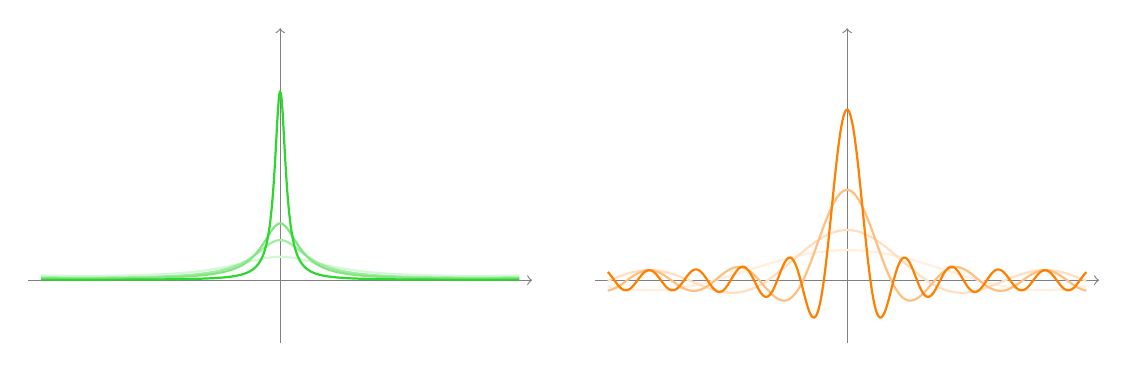
\begin{tikzpicture}[
	declare function = {
		poisson(\x, \r) = (1 - \r * \r) / (2 * pi * (1 - 2 * \r * cos (\x r) + \r * \r));
		dirichlet(\x, \n) = sin((\n + 0.5) * \x r) / (2 * pi * sin (0.5 * \x r));
	},
	scale = 0.8
]

\draw[->, gray] (-4, 0) -- (4,0);
\draw[->, gray] (0, -1) -- (0,4);

\foreach \r in {0.4, 0.6, 0.7, 0.9} {
	\pgfmathsetmacro{\colorpctg}{\r * \r * 100}
	\draw[thick, smooth, samples=300, variable=\x, domain=-3.8:3.8, green!80!black!\colorpctg!white]
		plot ({\x}, {poisson(\x, \r)});
}

\begin{scope}[xshift = 9cm]

\draw[->, gray] (-4, 0) -- (4,0);
\draw[->, gray] (0, -1) -- (0,4);
\foreach \n in {1, 2, 4, 8} {
	\pgfmathsetmacro{\colorpctg}{100 * \n / 8}
	\draw[thick, smooth, samples=300, variable=\x, domain=-3.8:3.8, orange!\colorpctg!white]
		plot ({\x}, {dirichlet(\x, \n)});
}
\end{scope}
\end{tikzpicture}
